% The talk's overview diagram, redrawn as vector graphics so it stays sharp on a
% large projection screen. It replaces an earlier screenshot of the same diagram.
%
% Build from this folder (the PDF lands here; auxiliary files go to the
% gitignored communication_drafts/build/ folder):
%   latexmk -pdf -auxdir=../build talk_hlg_111126_diagram_full.tex
% For a PNG outside the slides, e.g. 3840 pixels wide:
%   pdftoppm -r 412 -png -singlefile talk_hlg_111126_diagram_full.pdf talk_hlg_111126_diagram_full_4k
%
% Typeface: TeX Gyre Heros, a Helvetica/Arial-style sans, as in the original
% screenshot; the serif of the slides was tried and rejected here. Text colour:
% Moloch's dark teal, as in the slides.

% fix-cm makes the maths fonts scale freely, so the ↔ matches the large text.
\RequirePackage{fix-cm}
\documentclass[tikz, border=16pt]{standalone}

\usepackage[T1]{fontenc}
\usepackage{tgheros}
\renewcommand{\familydefault}{\sfdefault}
\usetikzlibrary{arrows.meta}

\definecolor{diagramtext}{HTML}{23373B}

% Two steps: talk_hlg_111126_diagram_partial.tex defines \diagrampartial and
% inputs this file.
% The parts marked "later" (abstract context, conjecture, and their arrows) are
% then drawn invisibly rather than left out, so both versions share one canvas and
% everything already shown stays in place when the full version replaces it.
\ifdefined\diagrampartial
  \tikzset{later/.style={opacity=0, text opacity=0}}
\else
  \tikzset{later/.style={}}
\fi

\begin{document}
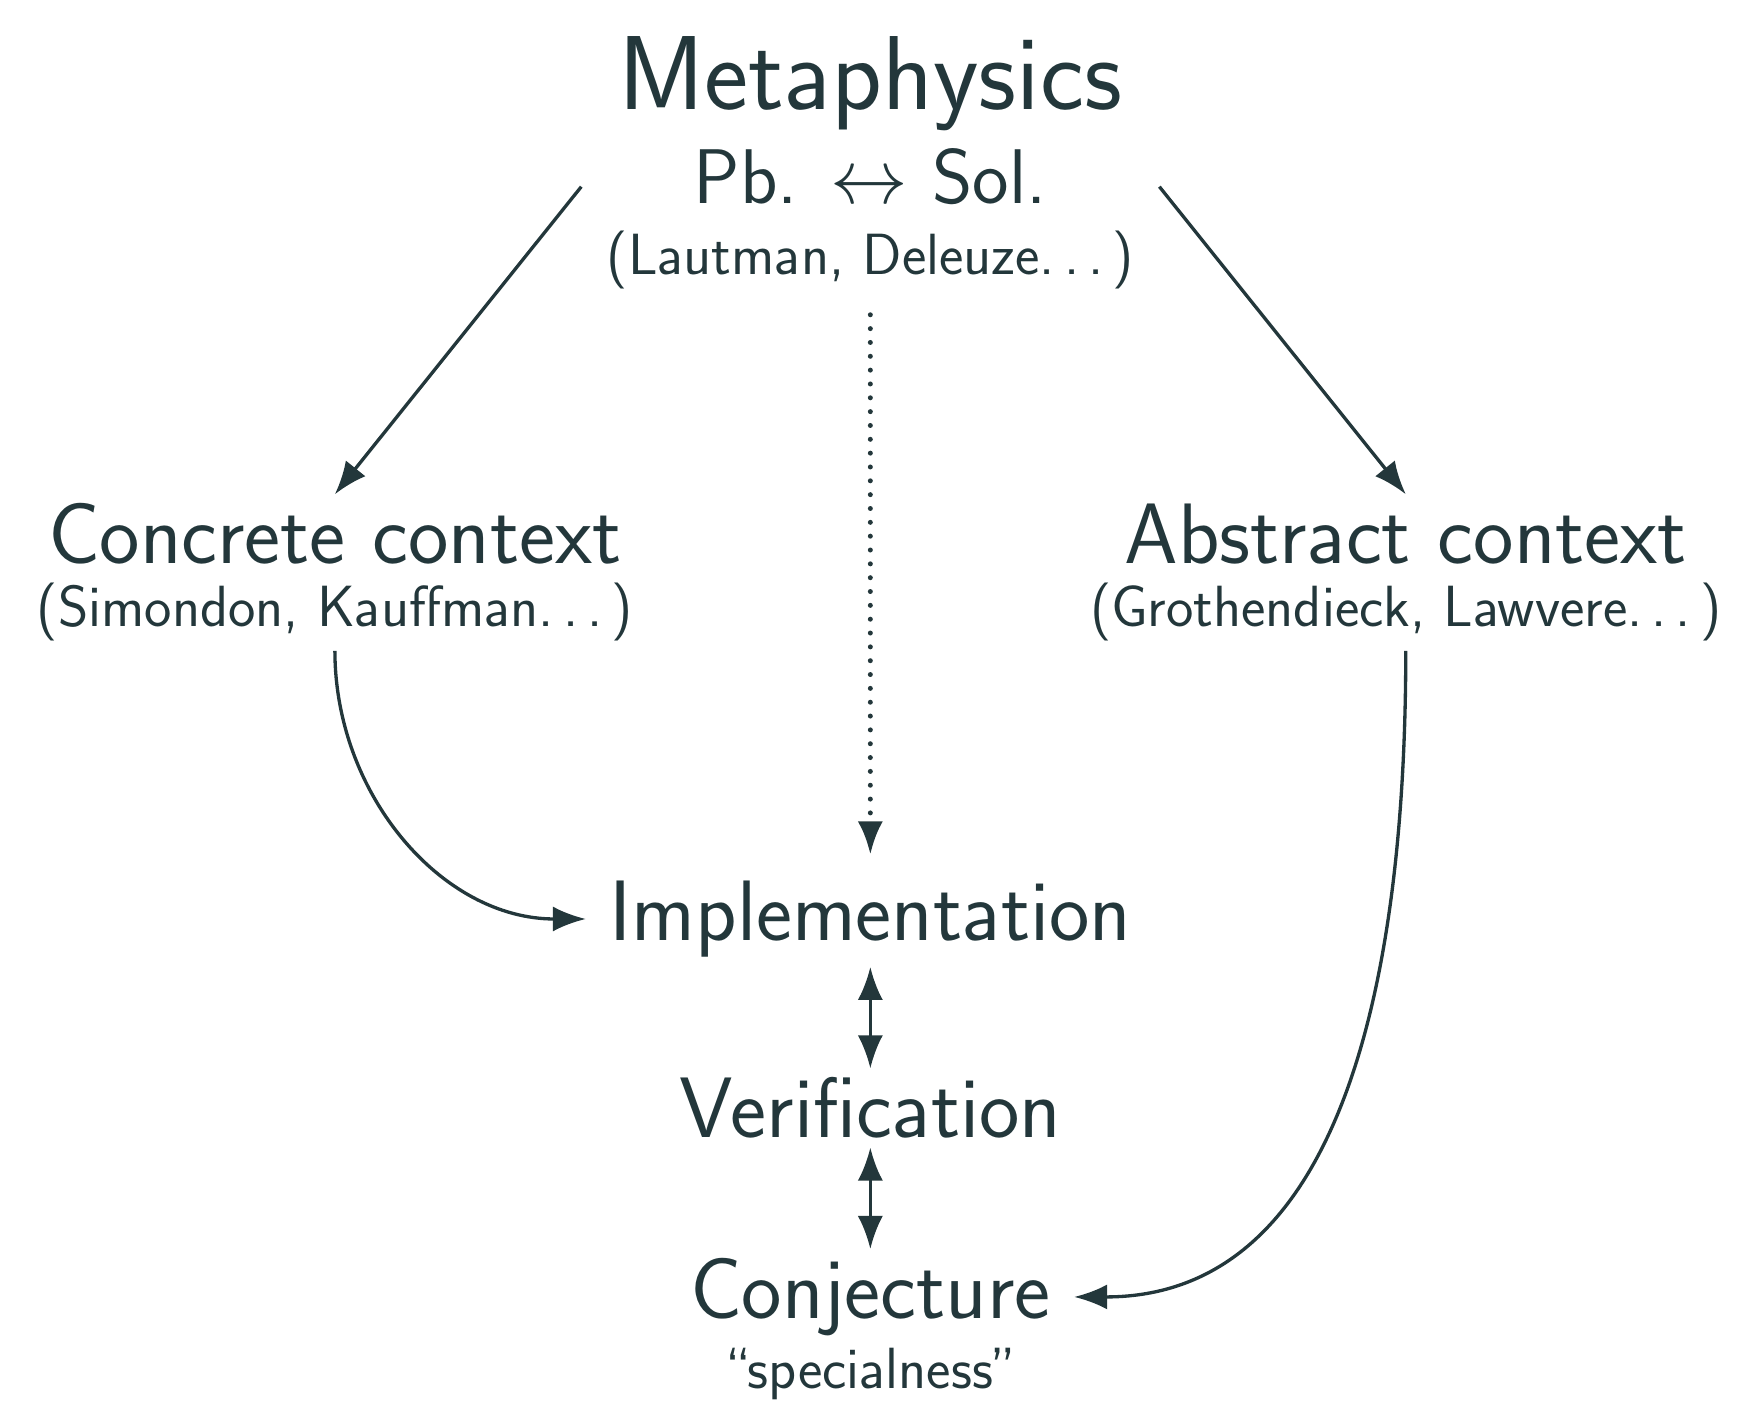
\begin{tikzpicture}[
    color=diagramtext,
    every node/.style={align=center, text=diagramtext},
    arrow/.style={-{Latex[length=4.2mm, width=3.2mm]}, line width=1.2pt},
    twoway/.style={{Latex[length=4.2mm, width=3.2mm]}-{Latex[length=4.2mm, width=3.2mm]}, line width=1.2pt},
    % Dotted and long, so the link from metaphysics to implementation reads as
    % indirect at a glance.
    dottedarrow/.style={arrow, line width=1.8pt, dash pattern=on 0pt off 5pt, line cap=round},
  ]

  \node (metaphysics) at (0, 0) {%
    {\fontsize{38}{44}\selectfont Metaphysics}\\[6pt]
    {\fontsize{28}{33}\selectfont Pb. $\leftrightarrow$ Sol.}\\[9pt]
    {\fontsize{21}{25}\selectfont (Lautman, Deleuze…)}%
  };

  \node (concrete) at (-6.8, -5.2) {%
    {\fontsize{31}{37}\selectfont Concrete context}\\[6pt]
    {\fontsize{21}{25}\selectfont (Simondon, Kauffman…)}%
  };

  \node[later] (abstract) at (6.8, -5.2) {%
    {\fontsize{31}{37}\selectfont Abstract context}\\[6pt]
    {\fontsize{21}{25}\selectfont (Grothendieck, Lawvere…)}%
  };

  \node (implementation) at (0, -9.6) {\fontsize{31}{37}\selectfont Implementation};
  \node (verification) at (0, -12.0) {\fontsize{31}{37}\selectfont Verification};
  \node[later] (conjecture) at (0, -14.4) {\fontsize{31}{37}\selectfont Conjecture};
  % A separate node, so the arrows still meet "Conjecture" itself.
  \node[later, anchor=north, inner sep=0pt] at ([yshift=-1pt]conjecture.south)
    {\fontsize{21}{25}\selectfont ``specialness''};

  \draw[arrow] (metaphysics.west) ++(-0.2, -0.3) -- (concrete.north);
  \draw[arrow, later] (metaphysics.east) ++(0.2, -0.3) -- (abstract.north);
  \draw[dottedarrow] (metaphysics.south) ++(0, -0.2) -- ([yshift=6pt]implementation.north);

  \draw[arrow] (concrete.south) to[out=-90, in=180] ([xshift=-5pt]implementation.west);
  \draw[arrow, later] (abstract.south) to[out=-90, in=0] ([xshift=5pt]conjecture.east);

  \draw[twoway] (implementation.south) -- (verification.north);
  \draw[twoway, later] (verification.south) -- (conjecture.north);

\end{tikzpicture}
\end{document}
